\section{Results}
Fifty whole-heart models
\replaced[id=PLOS, comment={Reviewer: cohort overview figure moved to supplement; cited as S1 Fig.}]{(\ref{fig:s1-hearts} Fig)}{(Figure~\ref{fig:hearts})}
were created, each including EP and mechanics simulations described in Section~\ref{sec:simulations}.
All simulations were performed with the same parameters for each model.
Therefore, the differences in simulations between sexes reported below relate to 
differences in anatomy.
% \paragraph{Descriptive statistics.}
We first examined the distributions of all core metrics across sex and condition.
A full table of means and standard deviations is provided in \replaced[id=PLOS, comment={EM: PLOS-style SI citation}]{S2 Data}{the Supplementary Material}.
We found no significant difference in age between males and females
(M: $53.4\pm15.0$\,y; F: $54.6\pm10.7$\,y; $p=0.75$). 
% % supplementary material: summary_table.xlsx 

\paragraph{Geometric characterization and correlation with simulation outputs.}
Geometric metrics stratified by sex and condition are provided in 
\replaced[id=PLOS, comment={PLOS: S1 Table form}]{\ref{tab:s1-geometric-characteristics} Table}{Supplementary Table~\ref{tab:s1-geometric-characteristics}}. 
Heart failure patients exhibited substantially larger chamber volumes 
compared to controls, with male HF patients showing the most pronounced dilation 
(LV: $289 \pm 88$~mL vs control: $180 \pm 36$~mL, $p<0.001$). Myocardial wall 
volume scaled with anatomical size, ranging from $263 \pm 37$~cm$^3$ 
in female controls to $396 \pm 75$~cm$^3$ in male HF patients.

Geometric variables showed strong correlations with simulation outputs 
(\replaced[id=PLOS, comment={PLOS/REV: S3 Fig (renumbered after hearts moved to S1)}]{\ref{fig:s3-correlation-heatmap} Fig}{Supplementary Figure~2}).
Chamber volume was the strongest predictor of 
volume change during passive inflation ($\rho = 0.96$ for LV, $p < 0.001$), 
indicating that larger ventricles exhibit greater absolute compliance under 
uniform material properties. Myocardial wall volume correlated strongly with 
activation times ($\rho = 0.87$ for TAT$_{\mathrm{RV}}$, $\rho = 0.85$ for 
TAT$_{\mathrm{V}}$, both $p < 0.001$), reflecting the expected increase in 
conduction path length with anatomical size. Notably, cross-chamber geometric 
correlations were observed, such as RV volume predicting LV activation time 
($\rho = 0.81$, $p < 0.001$), consistent with whole-heart anatomical coupling.

% Reviewer request: cohort overview figure (fig:hearts) moved to supplement as S1 Fig.
% See sections/supp/s_fig1_hearts.tex; label is now fig:s1-hearts.


% \subsection{Clinical literature metrics.}
Next, we assessed model volumes and the outputs of the EP and mechanics simulations.
In each case, we report the results from the two-way ANOVA and the post-hoc tests, showing 
the effect sizes. 
Where no interaction was present, we examined independent effects.
In both cases, only statistically significant results after FDR correction are reported here.
Effect sizes were computed using Cohen’s $d$ and are visualised in 
\replaced[id=PLOS, comment={PLOS: Fig (no period)}]{Fig}{Figure}~\ref{fig:cohen-big-effects}.

% \paragraph{\LA volume.} $\VOL{LA}$ had a significanfly higher mean in \HF\ patients,
\paragraph{\LV\ volume.} 
$\VOL{LV}$ was significantly larger in \HF\ patients and showed a significant interaction 
($p<0.05$ in ANOVA and all post-hoc comparisons).
For all but three male controls, the \LV\ volumes fall within the normal range 
($[109,218]$~mL)
compared to the UKBB reference values~\cite{petersen-2017-reference}.
Similarly, female controls also fall mostly within their corresponding normal range
($[88,161]~mL$).
We display the results in \replaced[id=PLOS, comment={PLOS: Fig (no period)}]{Fig}{Figure}~\ref{fig:validation-volumes}.
The effects sizes were also large between \HF\ and control groups, but they were much 
larger in males than in females, for instance, 
interactions involving females ranged between $0.9<d<1.17$, 
while interactions involving males were higher than $d>1.4$ 
($p<0.05$ in all cases, \replaced[id=PLOS, comment={PLOS: Fig (no period)}]{Fig}{Figure}~\ref{fig:cohen-big-effects}(a)).

\begin{figure}[hbpt]
    \centering
    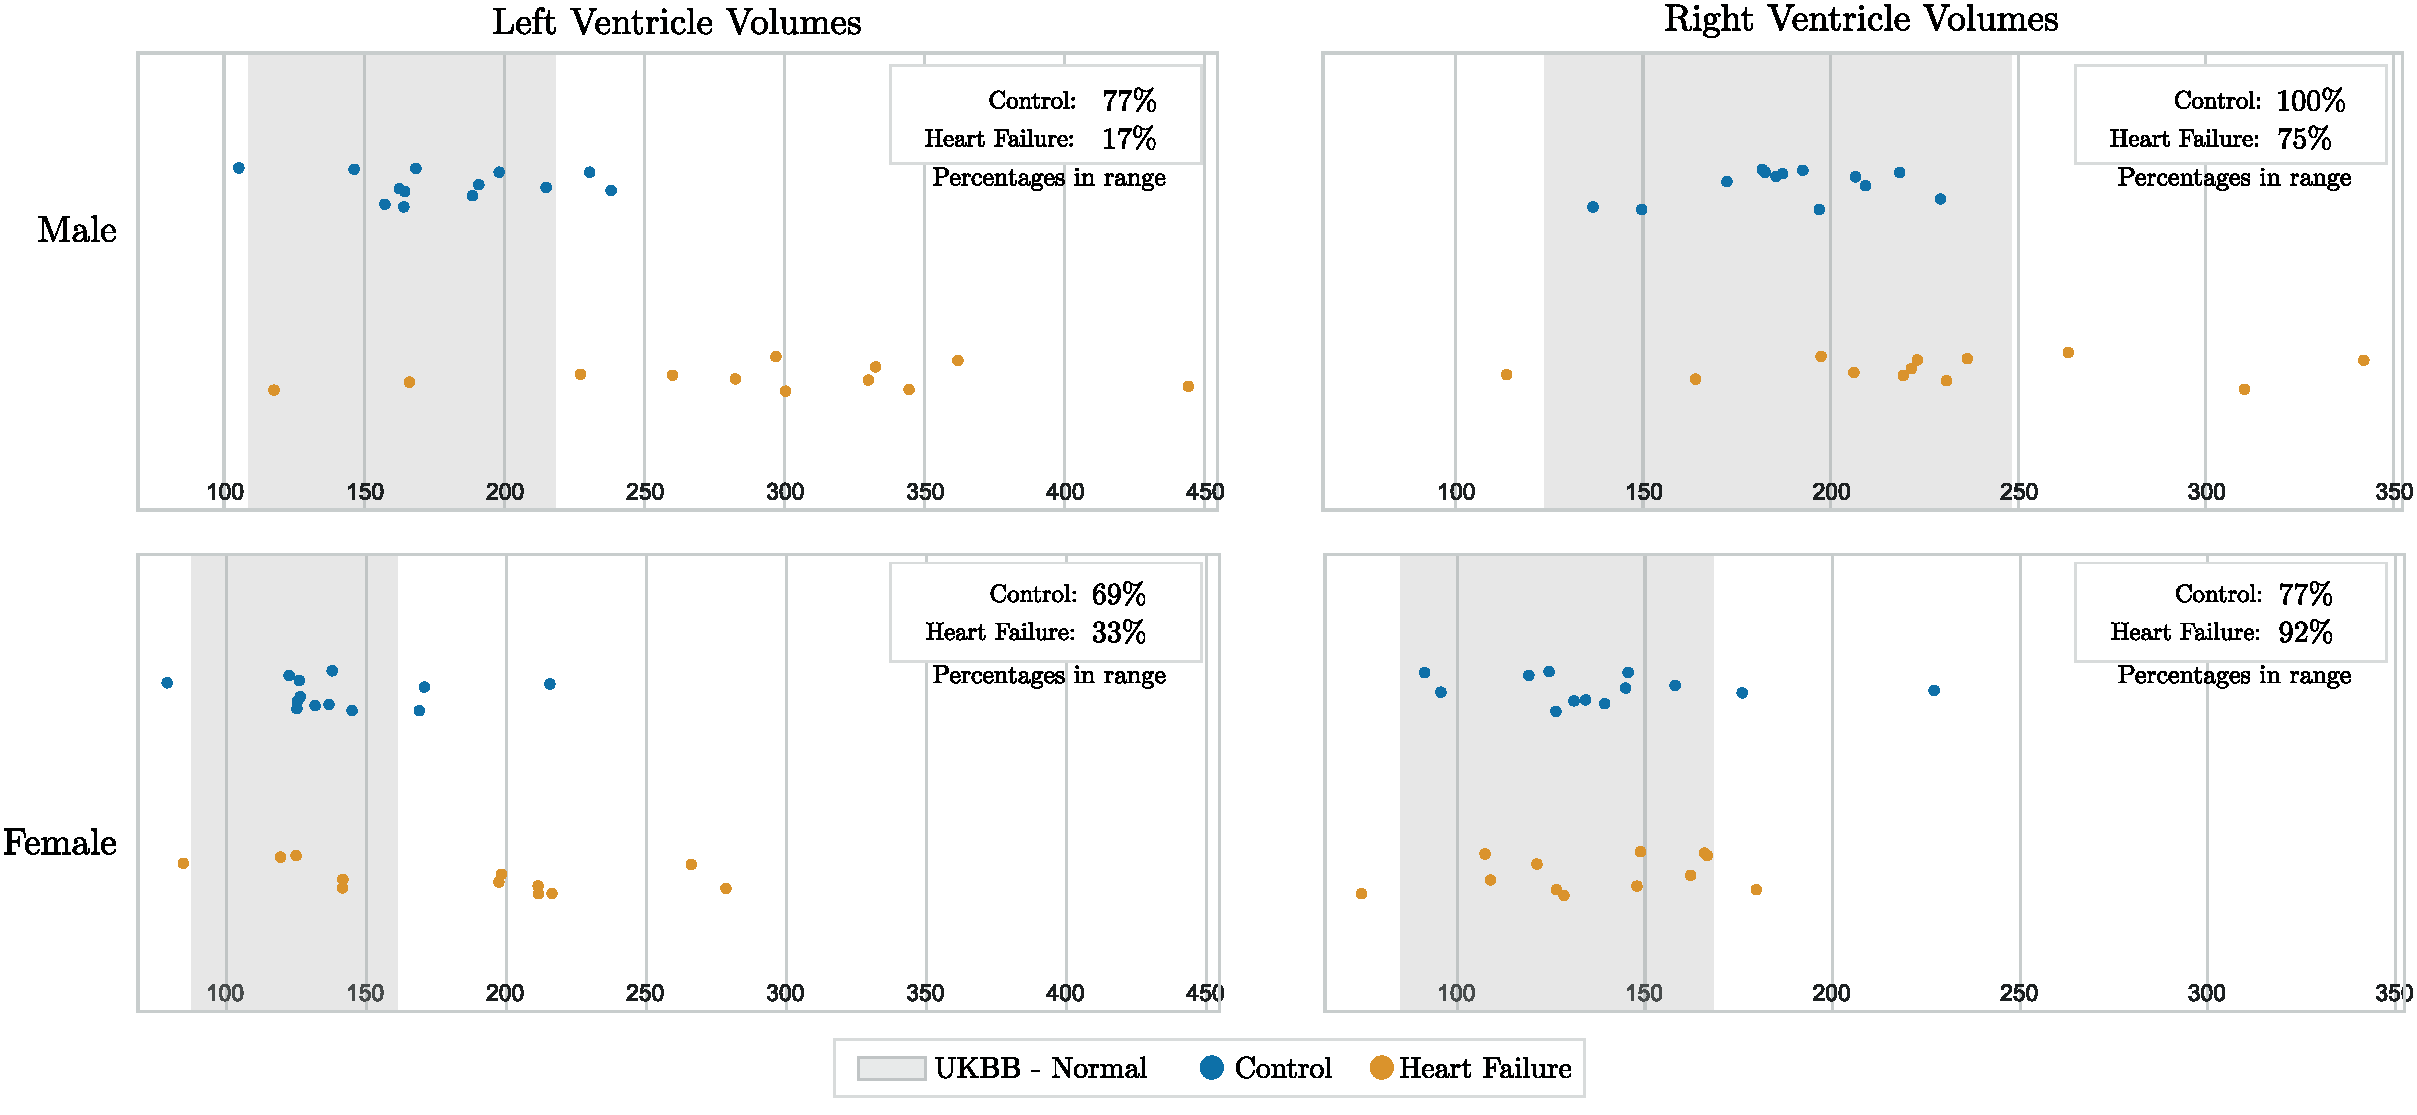
\includegraphics[width=\textwidth]{pics/fig6_results-validation-volumes-improved.pdf}
    \caption[Comparison vs clinical literature values and ranges from UKBB.]{
        \textbf{Comparison of measured ventricle volumes from the virtual cohort with}
        clinical literature values and ranges from UKBB.
        The UKBB normal ranges are defined as measurements within the 95\% prediction interval
        of the study by~\cite{petersen-2017-reference}. 
        Two graphs, corresponding to the \LV\ and \RV\ metrics and reference volumes. 
        Each plot is separated by sex and coloured by condition, with Controls in blue and 
        Heart Failure in orange.
        Normal ranges are shown as greyed areas, and exceeding the upper limit of the
        reference range may indicate pathological ventricular dilation. 
        Percentages of each group within the UKBB normal range are displayed in the legend.
    }
    \label{fig:validation-volumes}
\end{figure}
% ()
\paragraph{Volume change in the \LV.}
We used volume change as a surrogate for stiffness. 
\LV volume change was significantly larger in males compared to females and in 
\HF\ patients compared to controls (both main effects with $p<0.01$), 
but we did not detect a significant sex~$\times$~condition interaction ($p=0.44$), 
indicating that sex and condition contribute independently to \LV\ volume change. 
The effect sizes were large, with $d=0.94, p<0.01$ for \HF\ vs controls, 
and $d=0.78, p<0.01$ for male vs female comparisons 
(\replaced[id=PLOS, comment={PLOS: Fig (no period)}]{Fig}{Figure}~\ref{fig:cohen-big-effects}b).

\paragraph{Activation times.}
For ventricular $\TAT{V}$, no significant interaction was found between sex and condition ($p=0.76$), 
however, the independent effect sizes were large. 
First, $\TAT{V}$ was significantly longer in males compared to females ($d=1.4, p<0.01$), 
and in \HF\ patients compared to controls ($d=0.72, p=0.014$).
$\TAT{LA}$ showed a similar pattern. First, no significant interaction between sex and condition 
was found ($p=0.24$). Second, the independent effects were significant and moderate, showing 
prolonged activation times in \HF\ vs. controls ($d=0.62, p<0.05$) and prolonged activation 
in males vs. females ($d=0.59, p<0.05$). 

To assess the validity of using \TAT{} as a surrogate for QRS 
duration in the absence of torso modeling, we correlated simulated ventricular 
\TAT{} with recorded ECG QRS duration in cases where ECG data were available 
($n=33$ of $50$). In control hearts, \TAT{} showed a positive correlation with 
QRS duration (Pearson $r = 0.649, p < 0.005$, 
\replaced[id=PLOS, comment={PLOS/REV: S2 Fig (renumbered after hearts moved to S1)}]{\ref{fig:s2-tat-qrs} Fig}{Supplementary Figure~1}),
indicating that simulations using reference conductivity parameters provide an 
approximate anatomical surrogate for QRS duration, and that anatomical variation 
captures at least part of the inter-subject variability in activation time. 
In heart failure patients, no correlation was observed ($r = -0.127, p = 0.64$), 
consistent with the expected influence of pathological tissue properties 
(fibrosis, conduction blocks) that are not represented in our standardised 
parameter set.

\paragraph{Normalised volume changes in \LV.}
$\deltaVolNorm{LV}$ showed a significant interaction in the ANOVA between sex and condition ($p<0.05$).
Post-hoc tests only showed effects sizes were significant when comparing
\begin{itemize*}
    \item[] Male \HF\ vs. male controls ($d=-1.33$),
    \item[] Male vs. female with \HF\ ($d=-1.09$),
\end{itemize*} 
both with $p<0.05$.

% The largest effects were consistently observed in the ventricular metrics, 
% particularly in right ventricular volume and activation time between sexes, and in 
% left ventricular volume between males with and without heart failure.

\begin{figure}[hbpt]
    \centering
    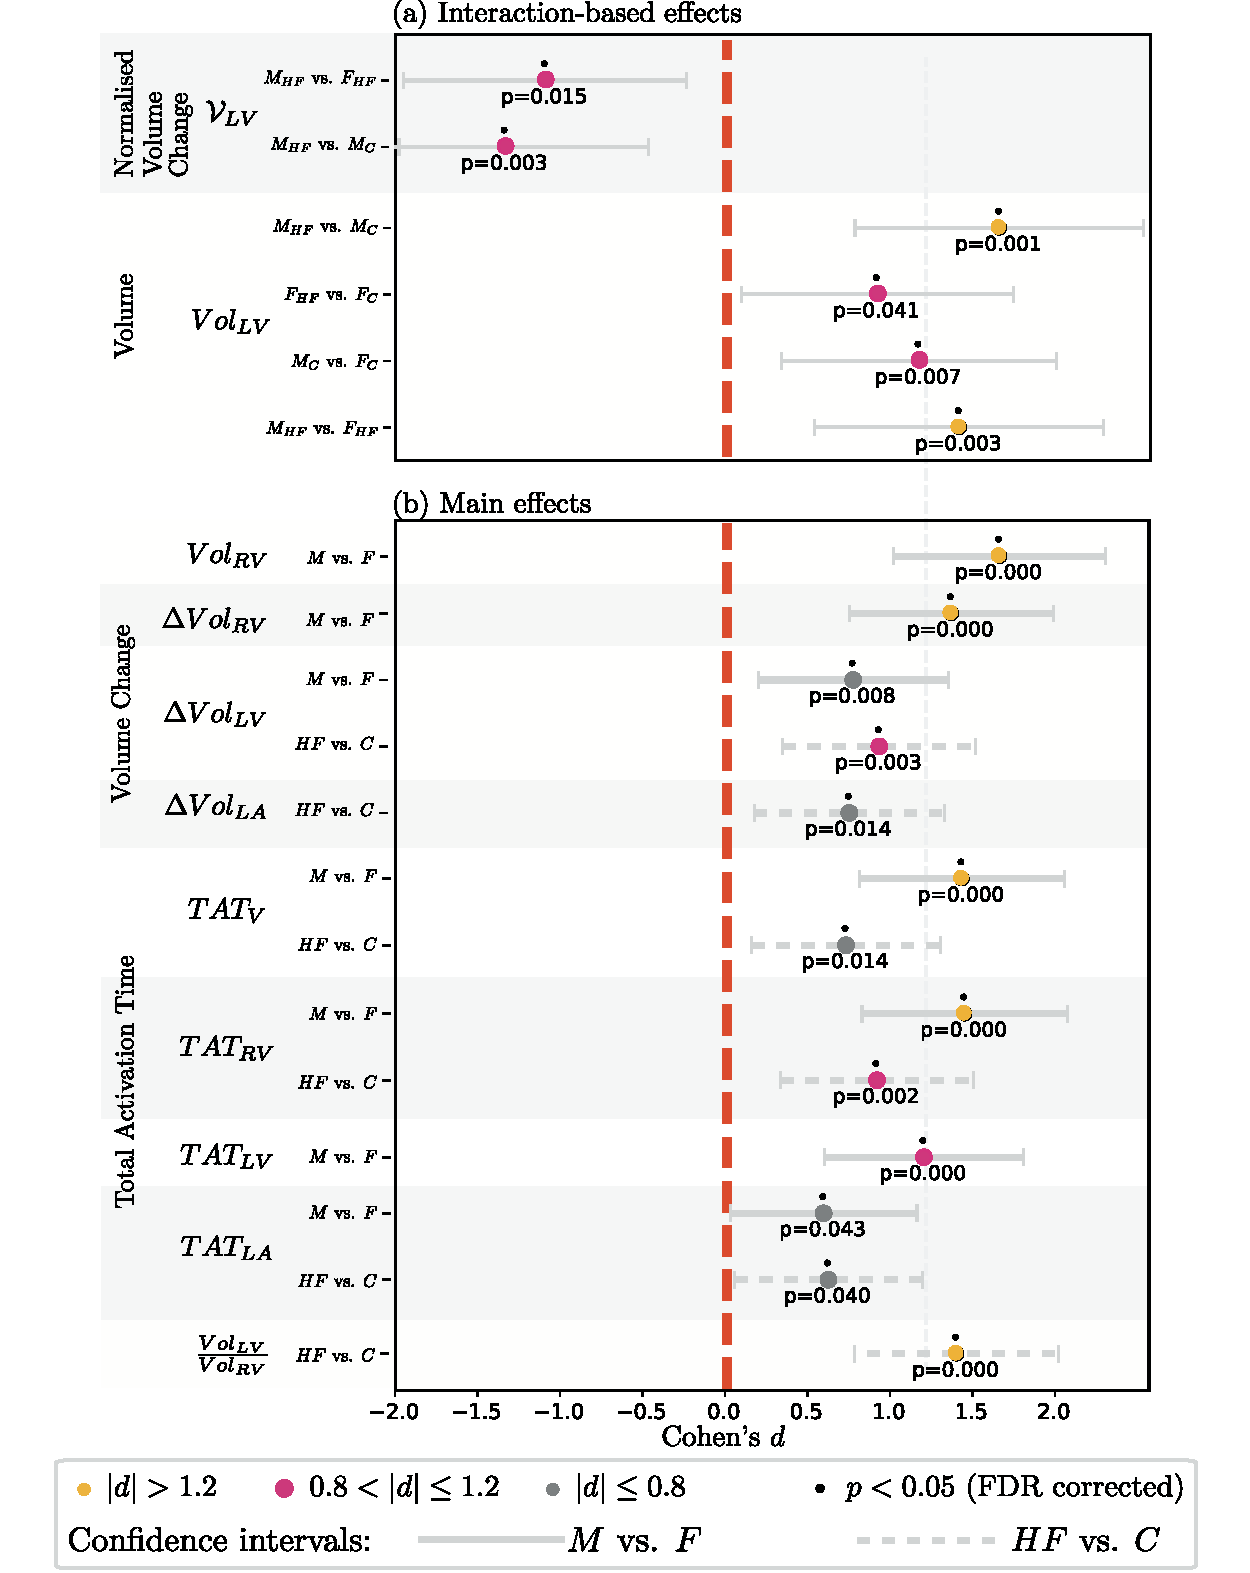
\includegraphics[width=\linewidth]{pics/fig7_cohen-big-effects.pdf}
    \caption[Large effect sizes from post-hoc comparisons.]{
        \textbf{Cohen’s d effect sizes from post-hoc comparisons following two-way ANOVA.}
        Metrics and group comparisons are displayed on the y-axis.
        This graph only shows effects with a high effect size and a corrected p-value $p<0.05$. 
        (a) Effect sizes for group comparisons performed when the Sex~$\times$~Condition 
        interaction was statistically significant, justifying 4 simple-effect post-hoc tests.
        (b) Effect sizes for marginal comparisons, when no significant interaction was found.
        Error bars line styles represent the comparison made: solid for sex, dotted for condition.
        \textit{Abbreviations}: M=Male, F=Female; C=Control, HF=Heart Failure; TAT=Total Activation time, 
        L/R=Left/Right, V=Ventricle.
    }
    \label{fig:cohen-big-effects}
\end{figure}